\chapter{Boosted Higgs identification}
\label{sec:05_jet_tagging}

In Part~\ref{part:hh}, we describe searches for the nonresonant SM and resonant BSM Higgs boson pair production, in the \bbvvq decay channel.
As discussed in Chapter~\ref{sec:01_higgs}, classifying the merged \hbb and \hyvv jets is a key component of these analyses.
Traditionally, jet-tagging involved hand-engineering high-level features, such as the jet mass, substructure variables, and secondary vertices, to manually define selections for such jets.
The advent of deep learning techniques, which are able to make effective use of low-level particle and vertex data, however, has revolutionized this process.

This is epitomized by the ParticleNet tagger~\cite{Qu:2019gqs}, described in Section~\ref{sec:05_hbb_tagger}, which uses a graph neural network (GNN) architecture to model individual jet constituents and their interactions, and has demonstrated strong performance on \hbb tagging (among other final states).
However, a similarly high performing classifier has not yet been developed for four-pronged \VVq jets.
In this chapter, we showcase the development of a new attention-based ParticleTransformer model~\cite{Qu:2022mxj} to identify such boosted \hvvq jets, which has proven to be a critical component of not only this analysis, but many ongoing boosted Higgs searches in CMS.
We additionally present a novel calibration method for the \hyvv tagger, which improves the systematic uncertainties on signal efficiency scale factors from 50\% using a previous proxy-based method~\cite{CMS:2022lqh} down to 16\%, representing a significant improvement in analysis sensitivity.

% We use the established mass-decorrelated (MD) version of this for tagging \hbb jets, as well as reconstructing the jet mass; and, since a similarly high-performing tagger has not yet been developed for \qqqq jets, we introduce a new transformer-based tagger for \hvvq jets.

\section{ParticleNet for \texorpdfstring{\bbbar}{bb}-jet tagging and mass regression}
\label{sec:05_hbb_tagger}

A ParticleNet model~\cite{CMS-DP-2020-002} has been trained to classify between background quark and gluon (QCD) jets and signal jets from a boosted spin-0 resonance (\PX) of mass varying between 15 and 250 \GeV and decaying into a pair of quarks, which are categorized into heavy and light flavors: $\PX\to\bbbar$, $\PX\to\ccbar$, and $\PX\to\qqbar$.
The mass of the resonance is varied to ensure the tagger cannot use it as a discriminating variable, thereby achieving mass decorrelation.
The model inputs are single AK8 jets with up to 100 PF candidates and 7 secondary vertices, each with 42 and 15 features, respectively, while the outputs are the probabilities of the jet to have originated from each of the individual training processes.

We focus on discriminating between $\PX\to\bbbar$ jets and QCD by using the $\TXbb$ discriminant, defined as:
\begin{equation}
    \label{eq:05_txbb}
  \TXbb = \frac{\PXbb}{\PQCD+\PXbb},
\end{equation}
where $P_{\mathrm{XYZ}}$ is the probability of class $\mathrm{XYZ}$ as outputted by ParticleNet.
This discriminator has shown to be highly performant for $\hbb$ vs QCD tagging, for example, in the CMS boosted $\HH\to\bbbb$ analysis~\cite{CMS:2022gjd}.

A similar model is also used to regress the mass of wide-radius jets.
It is trained on the same set of samples but trained to learn the ``true'' jet mass, defined as the \PX mass in the case of signal jets and the generator-level jet mass in the case of QCD jets.
A comparison of the traditional soft-drop algorithm~\cite{Larkoski:2014wba} (\msd) for mass reconstruction and the ParticleNet regressed mass (\mreg) is shown in Figure~\ref{fig:05_ak8jetmass_2018} for the \bbbar and \VV-candidate jets in the 2018 dataset for data, simulated background events, and a subset of the nonresonant and resonant signal samples.
We observe two significant benefits of the regressed mass:
1) the signal mass resolution is significantly improved, especially for the 4-pronged \VV jets; and
2) the regressed mass can recover jets that are too aggressively groomed by the soft-drop algorithm, as indicated by the peak at $0\GeV$ in \msd and lack thereof in \mreg.

\begin{figure}[htb!]
    \centering
    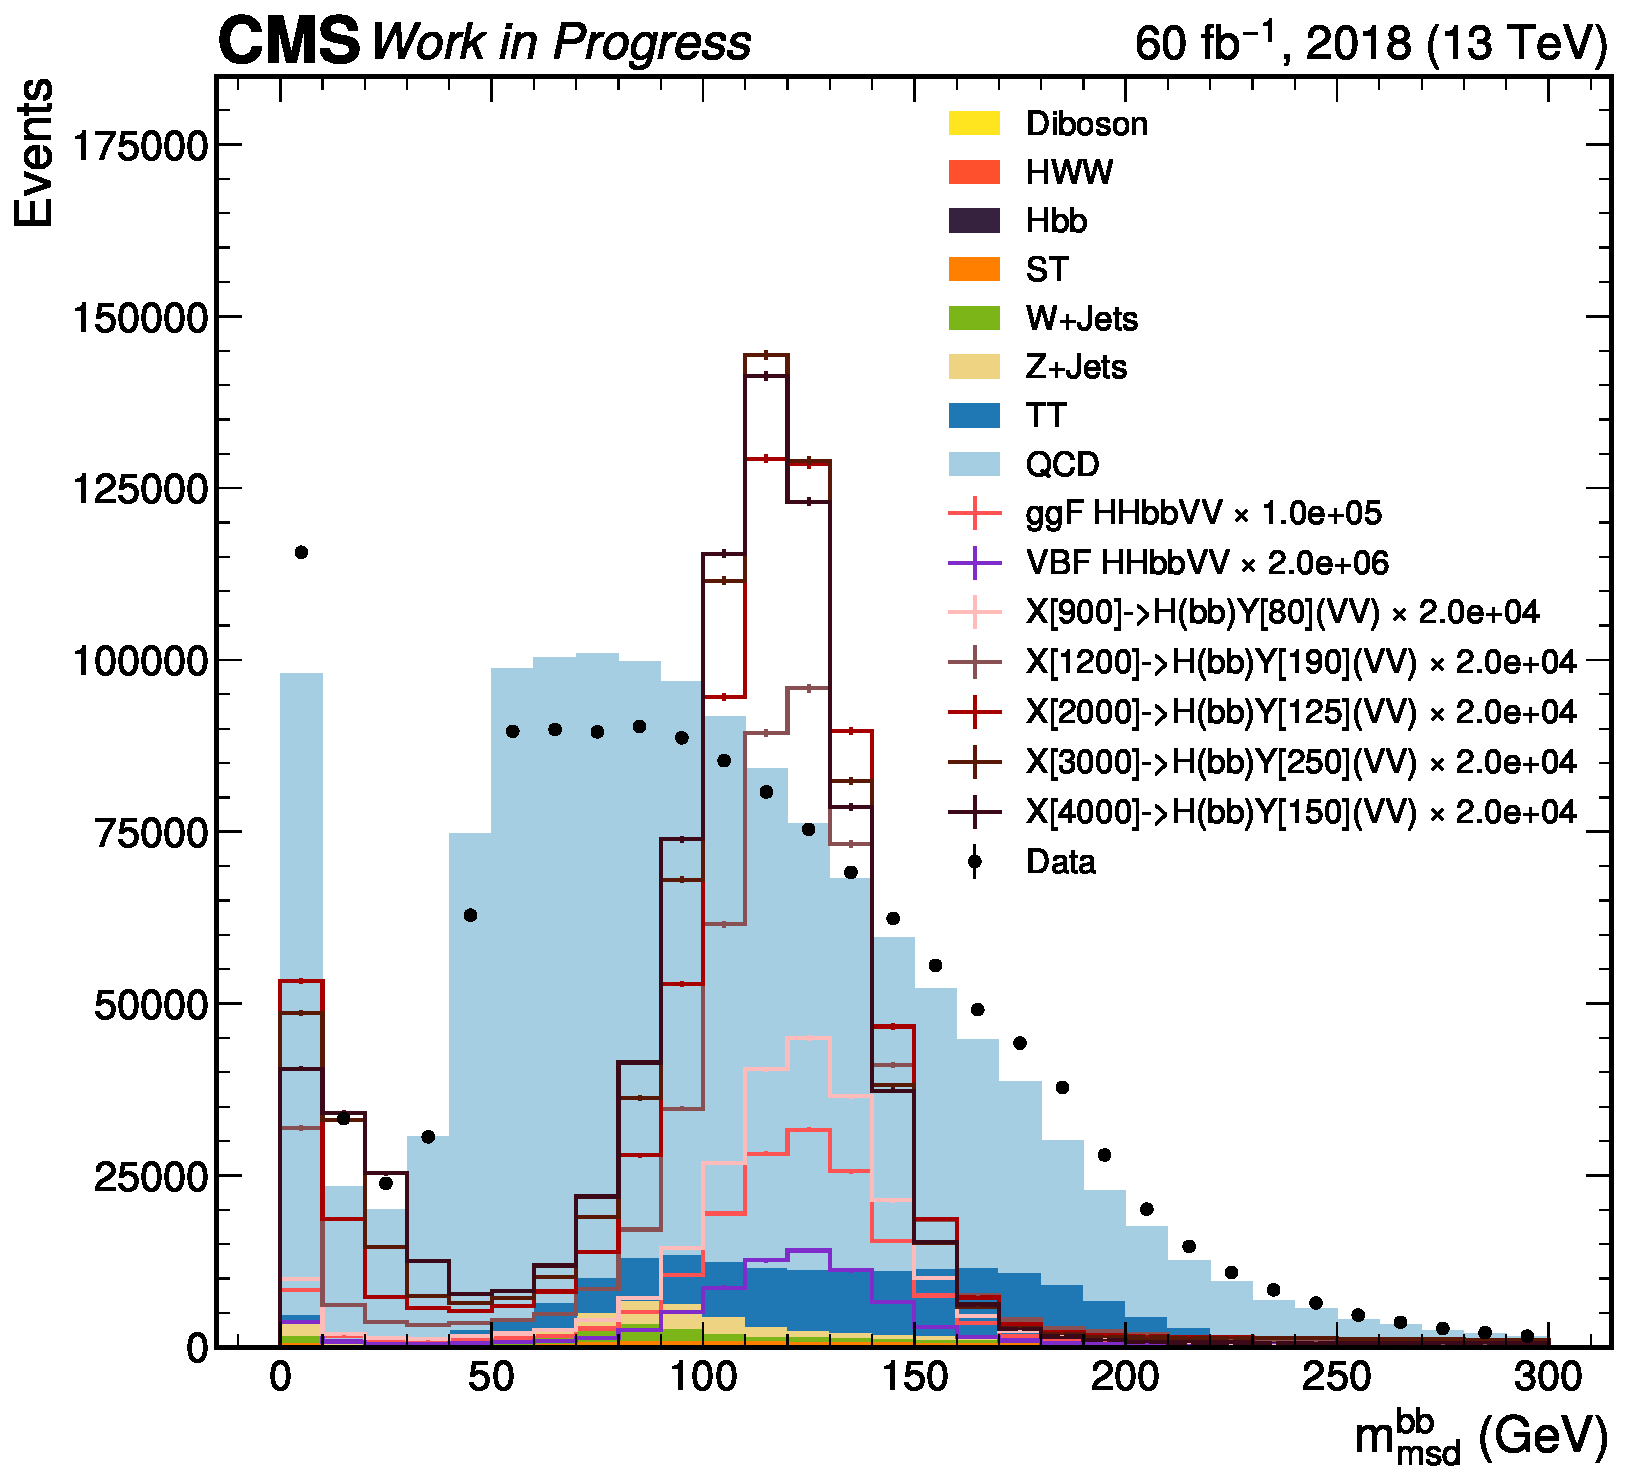
\includegraphics[width=0.49\textwidth]{figures/05-HH/jetmass/2018/bbFatJetMsd.pdf}
    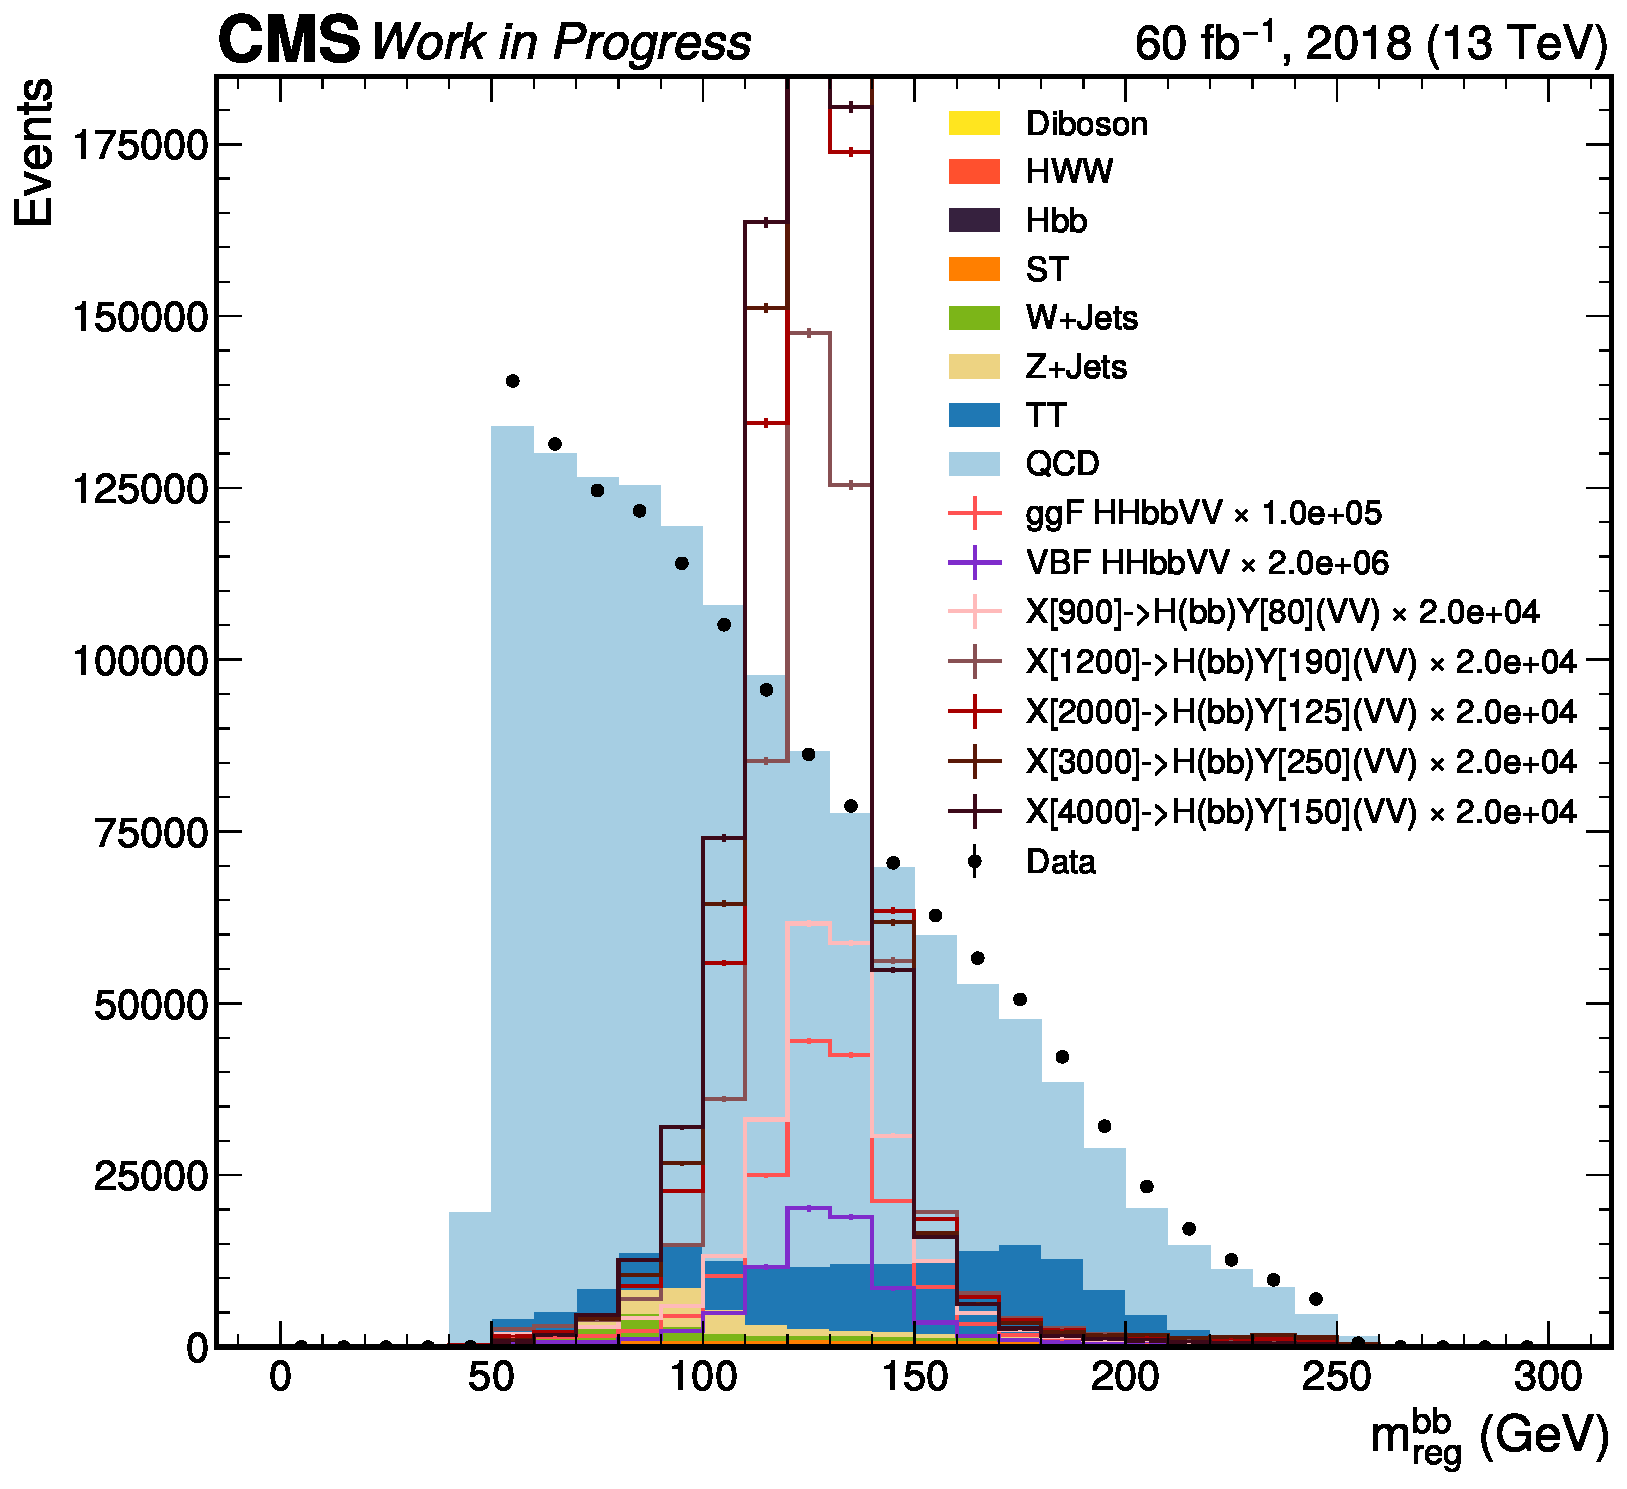
\includegraphics[width=0.49\textwidth]{figures/05-HH/jetmass/2018/bbFatJetParticleNetMass.pdf}
    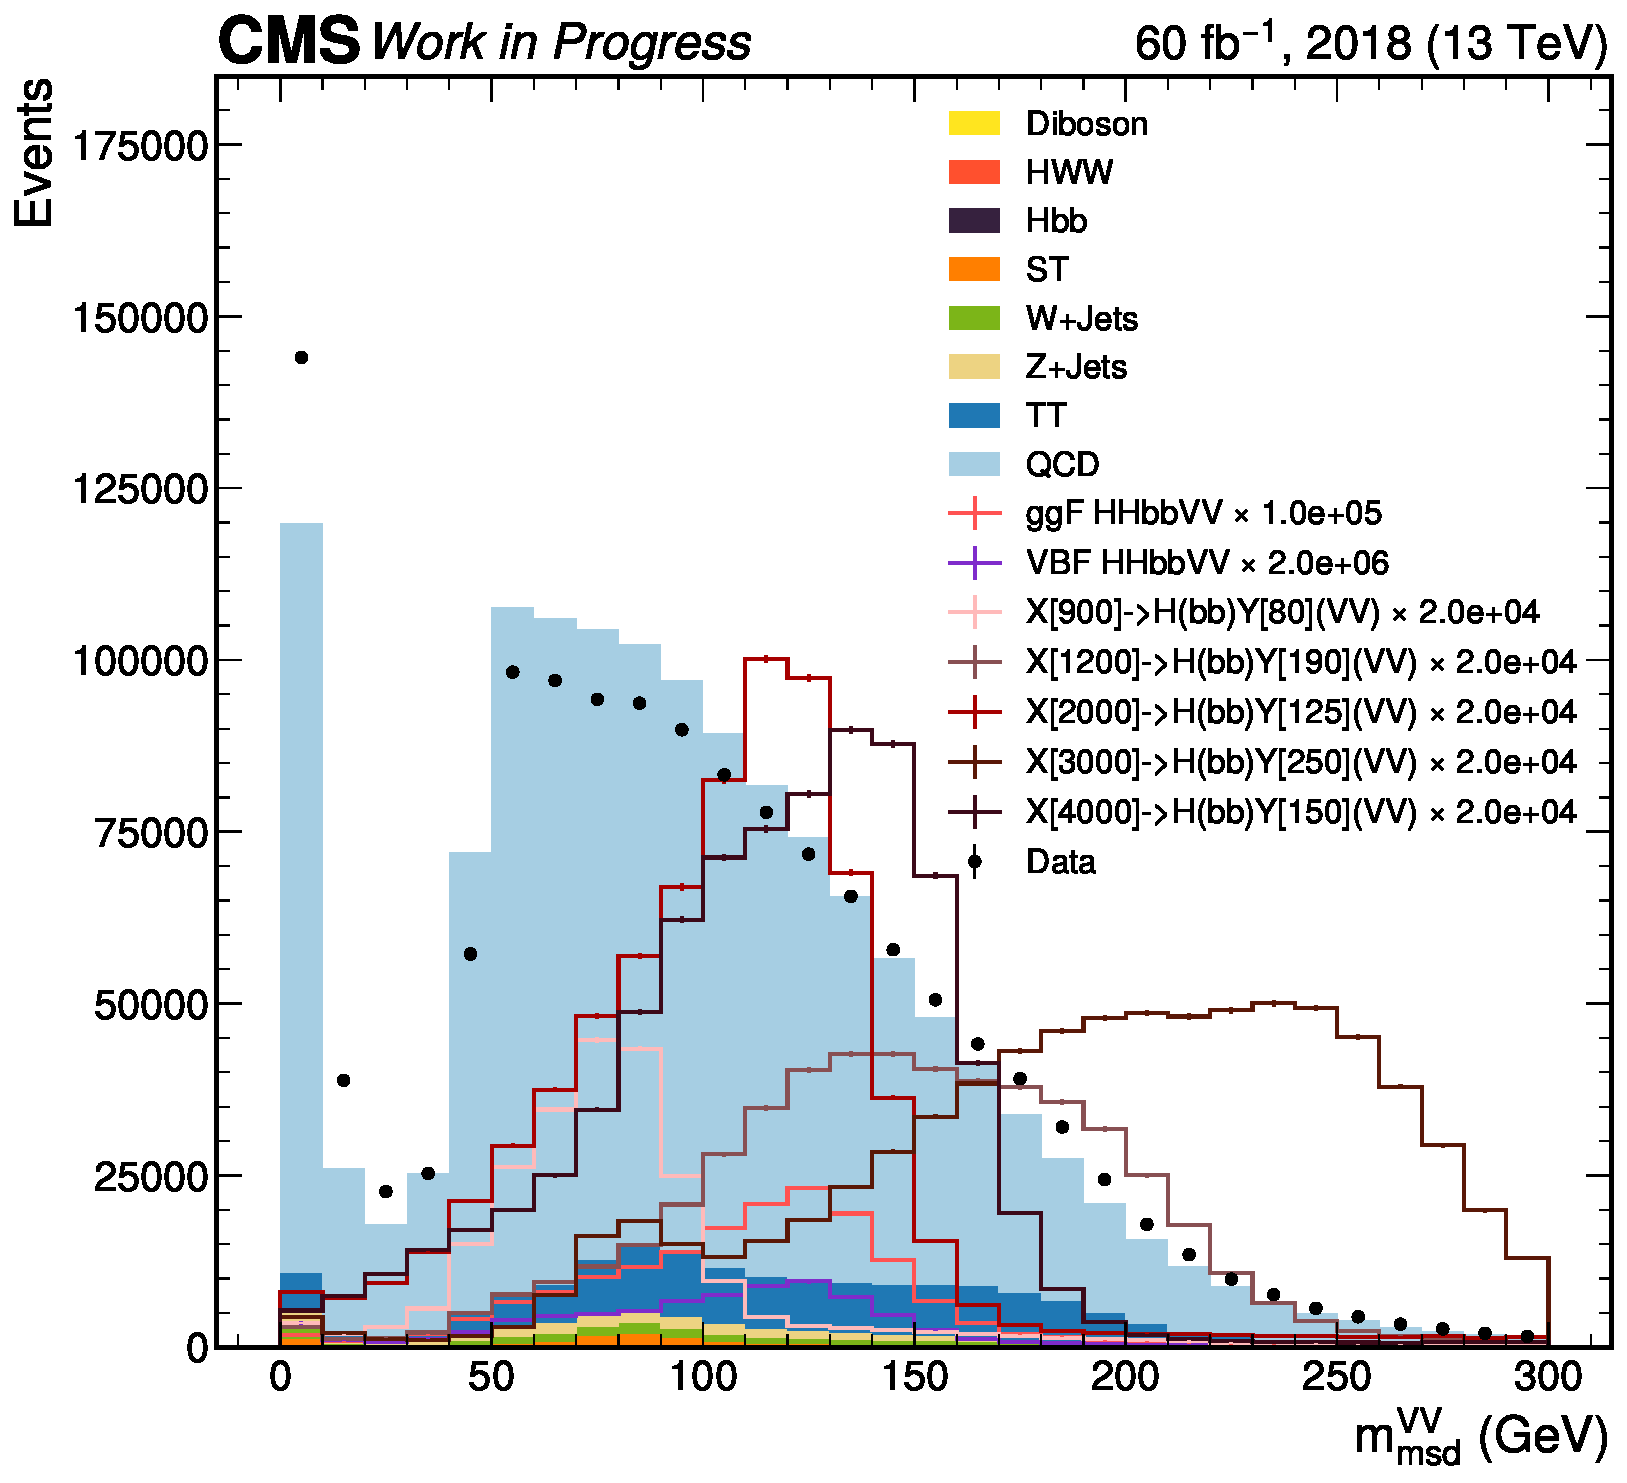
\includegraphics[width=0.49\textwidth]{figures/05-HH/jetmass/2018/VVFatJetMsd.pdf}
    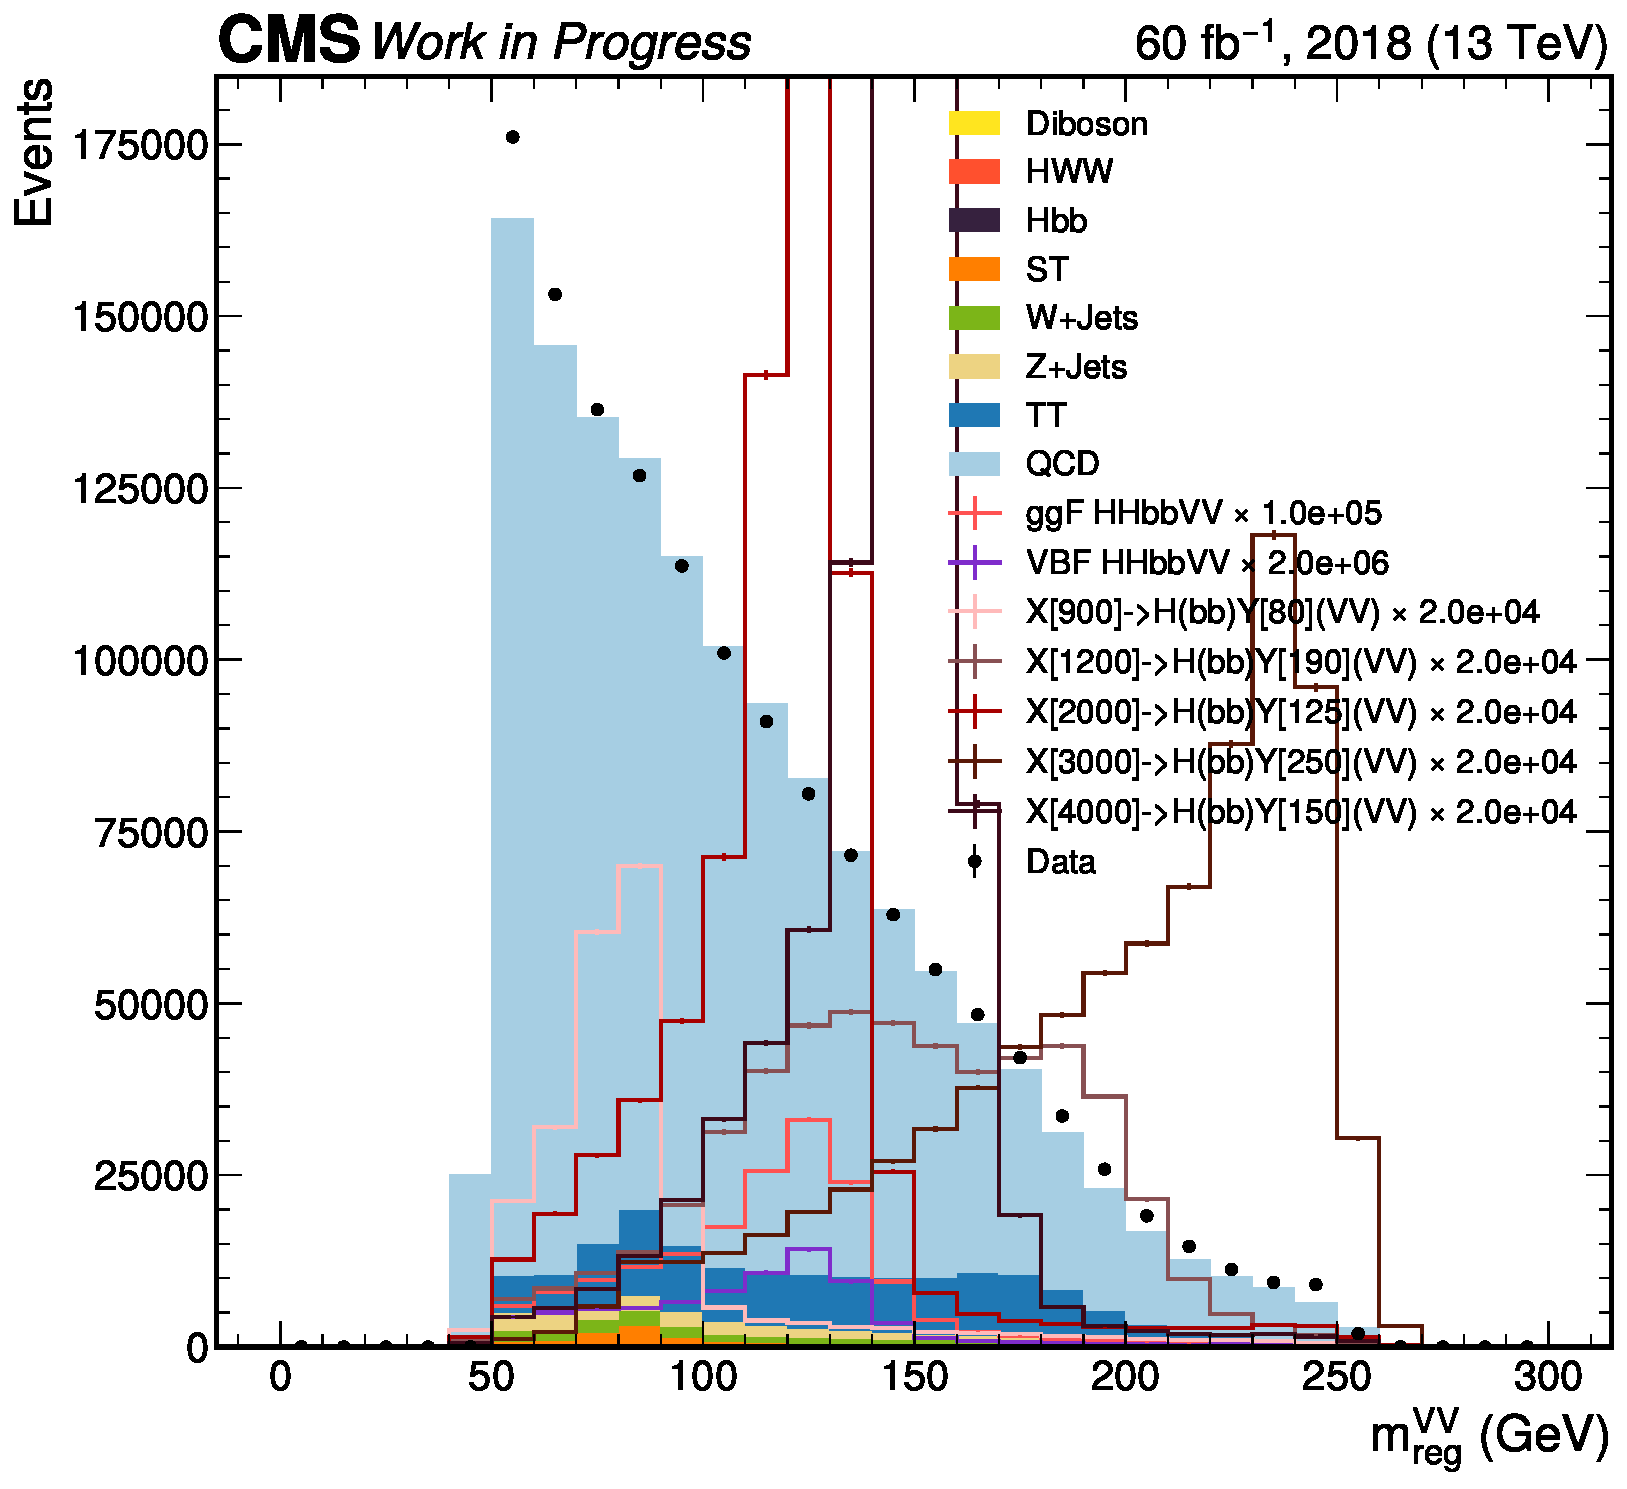
\includegraphics[width=0.49\textwidth]{figures/05-HH/jetmass/2018/VVFatJetParticleNetMass.pdf}
    \caption{Soft drop (left) and regressed (right) mass distributions for the \bbbar and \VV-candidate AK8 jets for 2018 data and simulated samples following a loose pre-selection for boosted jets.}
    \label{fig:05_ak8jetmass_2018}
\end{figure}

\section{GloParT for \texorpdfstring{\hyvv}{H/Y→VV} classification}
\label{sec:05_hww_tagger}

To target the \hyvvq jets, as well as several additional signatures, we introduce a new transformer-based model, based on the ParT~\cite{Qu:2022mxj} architecture, called ``Global Particle Transformer'' (GloParT).
It is trained to classify between background QCD jets and a wide variety of fully hadronic and semi-leptonic Higgs and top quark processes.
The full set of training classes is illustrated in Figure~\ref{fig:05_part_classes}.
As for the ParticleNet tagger, to achieve mass-decorrelation, the masses of Higgs- and top-quark-like resonances are varied in the training samples; specifically, Higgs-like topologies are simulated using spin-0 particles (\PG) decaying to \HH and top-quark-like topologies with \PG decaying to \ttbar, where the \PH and \PQt masses are varied between 15 and 250\GeV.
For \hvv decays, the \PW and \PZ boson masses are also varied, either linearly with the \PH mass---for SM Higgs boson searches such as the nonresonant \HH search, or independently, motivated by BSM scenarios such as the resonant \XHY search.

The final states for each process are grouped by the number of quarks and leptons per jet, and then further separated by heavy flavors.
Notably, fully hadronic \hvv jets are separated into 4- and 3-pronged jets (qqqq and qqq), to account for boosted jets which may not capture all four \VV daughter quarks.
The inputs to the model are AK8 jets with up to 128 PF candidates and 7 secondary vertices, with features listed in Table~\ref{tab:05_part_inputs}, and the outputs are the probabilities of the jet to have originated from each of the aforementioned processes and final states.

In the resonant analysis (and to evaluate the performance of the tagger for nonresonant signals), we focus on discriminating between the hadronic \hvv final states and top quark and QCD multijet backgrounds using the \THWW discriminator defined as
\begin{equation}
  \label{eq:05_thww}
  \THWW = \frac{\PHWWqqqq + \PHWWqqq}{\PQCD + \PTop + \PHWWqqqq + \PHWWqqq},
\end{equation}
where \PHWWqqqq, \PHWWqqq, \PQCD, and \PTop are the sum of the predicted probabilities of their respective sub-categories.
The performance of this discriminant on \VV-candidate jets passing loose a preselection for boosted jets is shown in Figure~\ref{fig:05_part_roc}.
In the nonresonant analysis, the raw \PHWWqqqq, \PHWWqqq, \PQCD, and \PTop are used as inputs to the BDT.

\begin{figure}[htb!]
    \centering
    \captionsetup{justification=centering}
    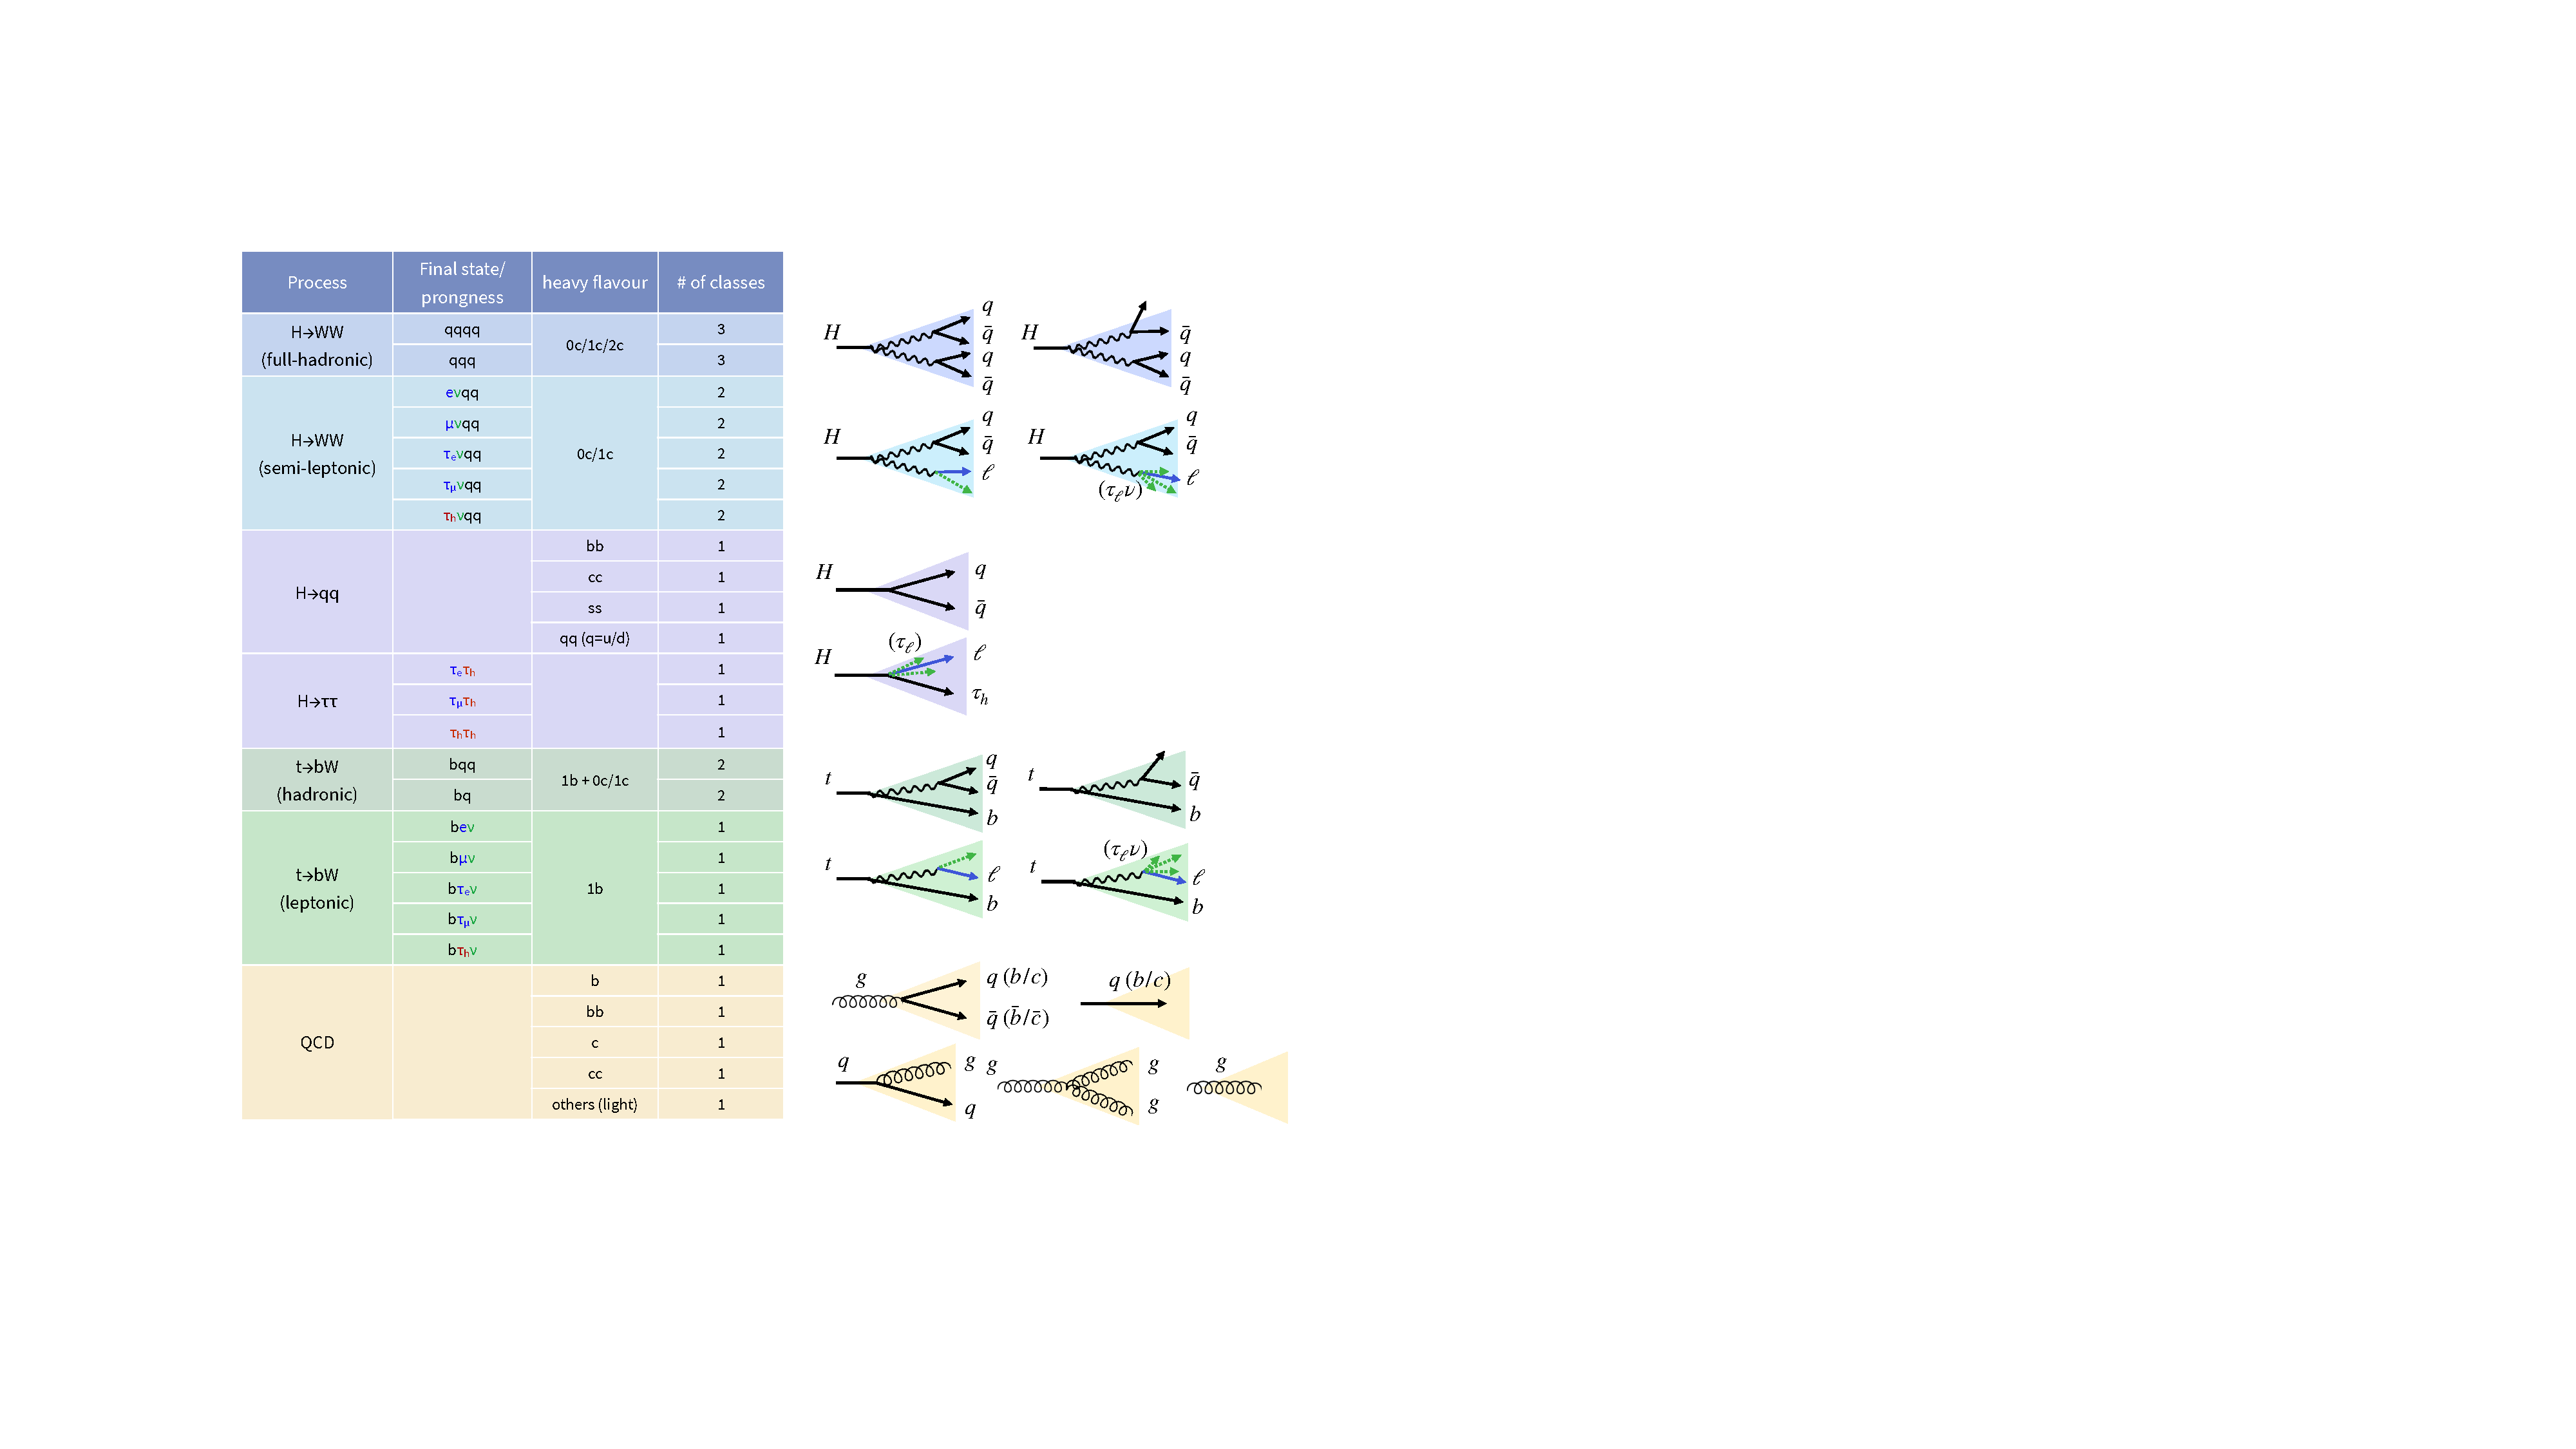
\includegraphics[width=0.8\textwidth]{figures/05-HH/part/classes_stage1.pdf}
    \caption{Full set of training jet classes for GloParT.}
    \label{fig:05_part_classes}
\end{figure}

\begin{table}[htb!]
    \begin{center}
    \caption{The complete set of input features into GloParT. Three types of inputs are considered: charged PF candidates, neutral PF candidates, and secondary vertices (SVs).}
    \label{tab:05_part_inputs}
    \resizebox*{\textwidth}{!}{
    \begin{tabular}{ll}
    \hline\hline
    Variable & Definition \\ \hline\hline
    \multicolumn{2}{c}{\textbf{charged PF candidates}}\\\hline
    $\log\pt$ & logarithm of the particle’s \pt \\
    $\log E$ & logarithm of the particle’s energy \\
    $\Delta\eta(\text{jet})$ & difference in pseudorapidity between the particle
    and the jet axis\\
    $\Delta\phi(\text{jet})$ & difference in azimuthal angle between the particle
    and the jet axis \\
    $|\eta|$ & absolute value of the particle's pseudorapidity\\
    $q$ & electric charge of the particle\\
    \texttt{isMuon} & if the particle is identified as a muon \\
    \texttt{isElectron} & if the particle is identified as an electron \\
    \texttt{isChargedHadron} & if the particle is identified as a charged hadron \\
    \texttt{pvAssociationQuality} & flag related to the association of the track to
    the primary vertices \\
    \texttt{lostInnerHits} & quality flag of the track related to missing hits on
    the pixel layers \\
    $\chi^2/dof$ & $\chi^2$ value of the trajectory fit normalized to the number of
    degrees of freedom \\
    \texttt{qualityMask} & quality flag of the track \\
    $d_z$ & longitudinal impact parameter of the track \\
    $d_z$/$\sigma_{d_{z}}$ & significance of the longitudinal impact parameter \\
    $d_{xy}$ & transverse impact parameter of the track \\
    $d_{xy}$/$\sigma_{d_{xy}}$ & significance of the transverse impact parameter \\
    $\eta_{\text{rel}}$ & pseudorapidity of the track relative to the jet axis \\
    $p_{\text{T,rel}}$ ratio & track momentum perpendicular to the jet axis,
    divided by the magnitude of the track momentum \\
    $p_{\text{par,rel}}$ ratio & track momentum parallel to the jet axis divided by
    the magnitude of the track momentum \\
    $d_{\text{3D}}$ &  signed 3D impact parameter of the track \\
    $d_{\text{3D}}/\sigma_{\text{3D}}$ & signed 3D impact parameter significance of
    the track \\
    \texttt{trackDistance} & distance between the track and the jet axis at their
    point of closest approach \\
    \hline\hline
    
    \multicolumn{2}{c}{\textbf{Neutral PF candidates}}\\\hline
    $\log\pt$ & logarithm of the particle’s \pt \\
    $\log E$ & logarithm of the particle’s energy \\
    $\Delta\eta(\text{jet})$ & difference in pseudorapidity between the particle
    and the jet axis\\
    $\Delta\phi(\text{jet})$ & difference in azimuthal angle between the particle
    and the jet axis \\
    $|\eta|$ & absolute value of the particle's pseudorapidity\\
    \texttt{isPhoton} & if the particle is identified as a photon \\
    \texttt{isNeutralHadron} & if the particle is identified as a neutral hadron \\
    \hline\hline
    \multicolumn{2}{c}{\textbf{For SVs within the jet cone}}\\\hline
    $\log\pt$ & logarithm of the SV \pt \\
    $m_{\text{SV}}$ & mass of the SV \\
    $\Delta\eta(\text{jet})$ & difference in pseudorapidity between the SV and the
    jet axis\\
    $\Delta\phi(\text{jet})$ & difference in azimuthal angle between the SV and the
    jet axis \\
    $|\eta|$ & absolute value of the SV's pseudorapidity\\
    $N_\text{tracks}$ & number of tracks associated with the SV \\
    $\chi^2/dof$ & $\chi^2$ value of the SV fit normalized to the number of degrees
    of freedom \\
    $d_{\text{2D}}$ &  signed 2D impact parameter (i.e., in the transverse plane)
    of the SV \\
    $d_{\text{2D}}/\sigma_{\text{2D}}$ & signed 2D impact parameter significance of
    the SV \\
    $d_{\text{3D}}$ &  signed 3D impact parameter of the SV \\
    $d_{\text{3D}}/\sigma_{\text{3D}}$ & signed 3D impact parameter significance of
    the SV \\
    \hline\hline
    \end{tabular}
    }
    \end{center}
    \end{table}

\begin{figure}[htb!]
    \centering
    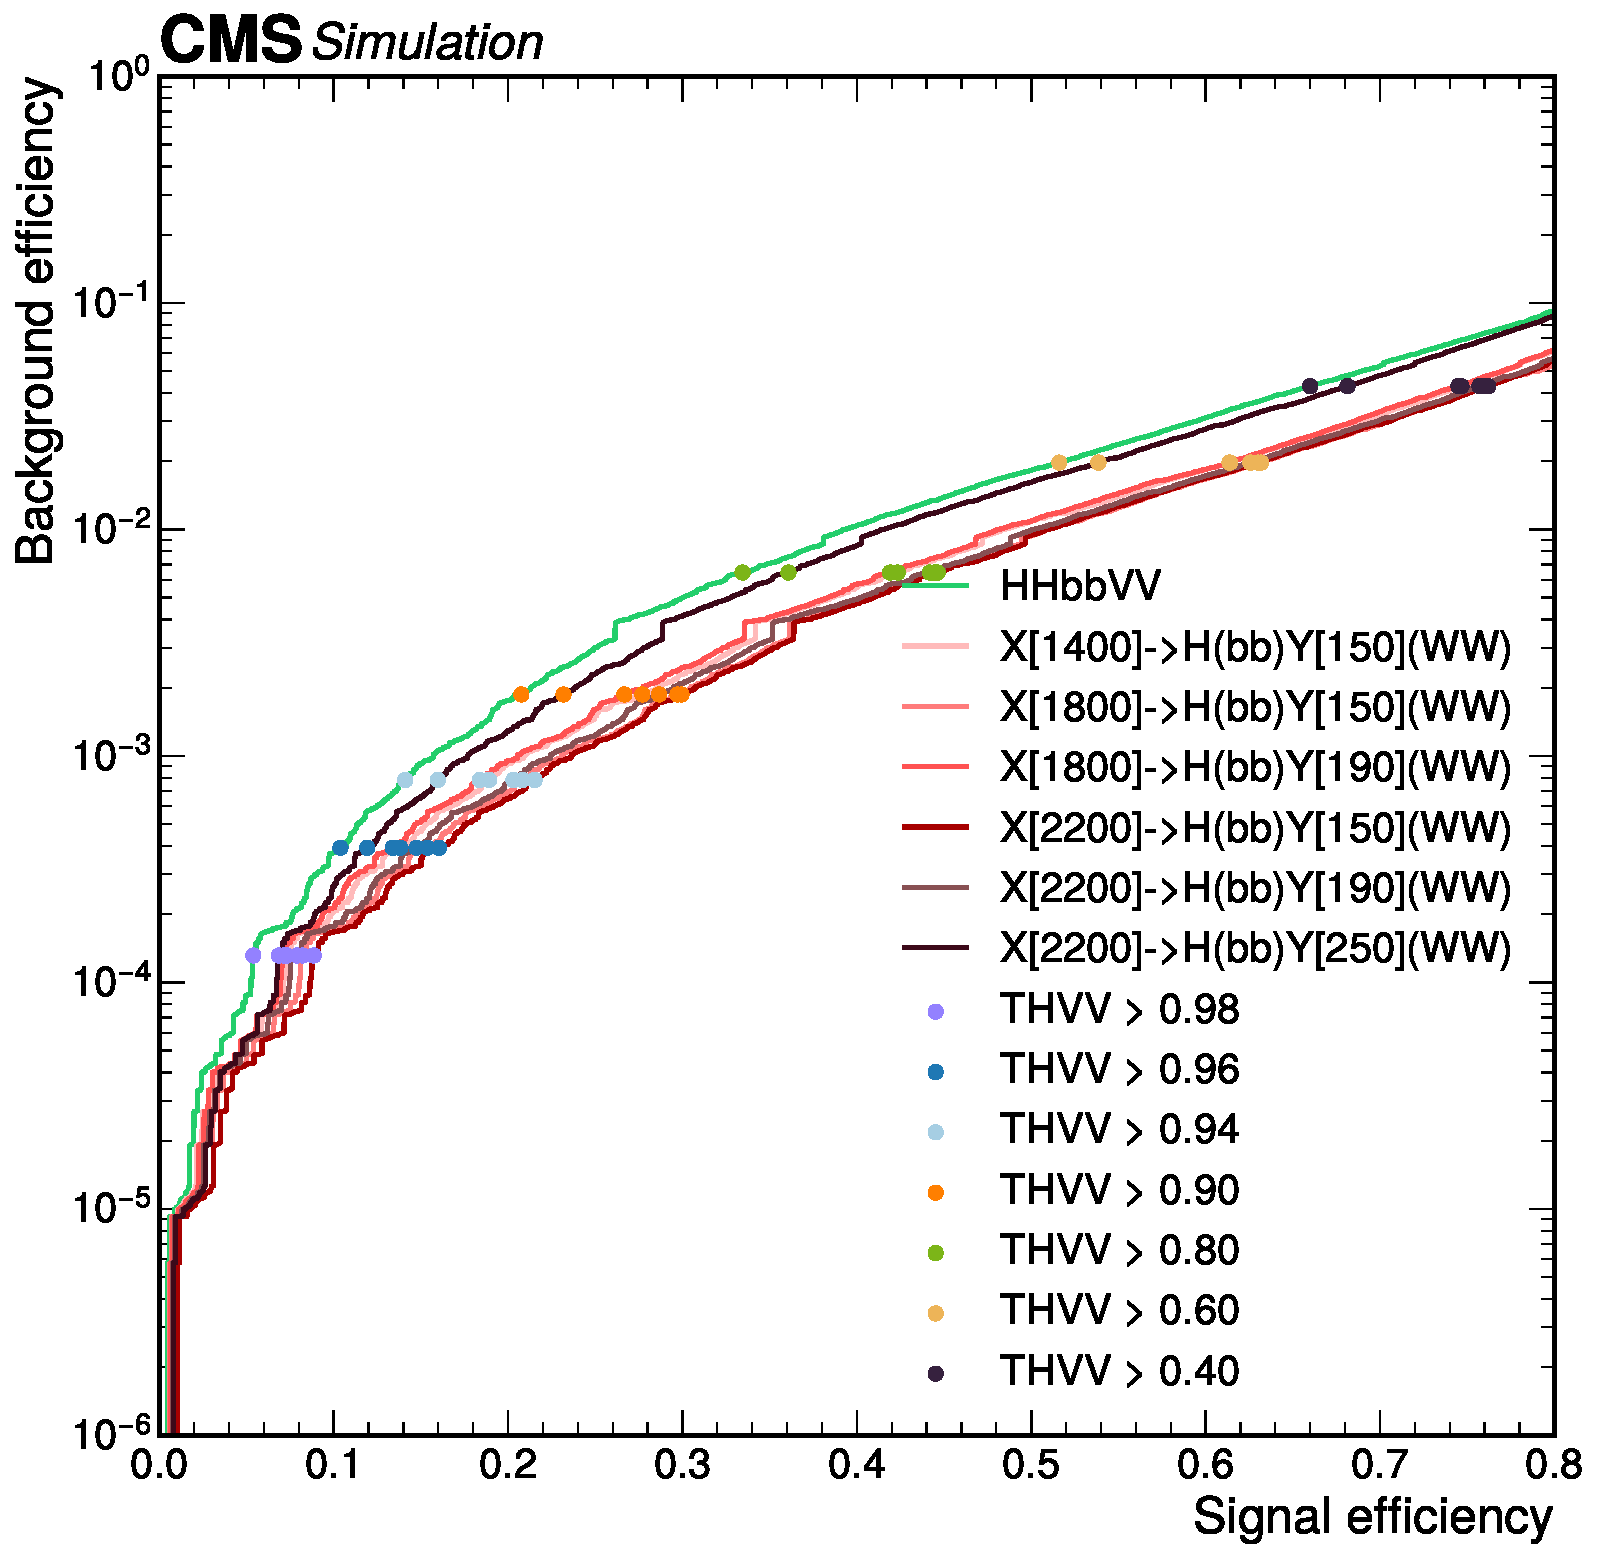
\includegraphics[width=0.6\textwidth]{figures/05-HH/part/roccurve_allsigs_thvv4qt_pt_300_3000.pdf}
    \caption{Receiver operating characteristic (ROC) curve for the \THWW discriminator on \VV-candidate jets passing the AK8 online and offline selections for a subset of nonresonant and resonant signals versus QCD and \ttbar backgrounds.}
    \label{fig:05_part_roc}
\end{figure}

\section{Calibrating \texorpdfstring{\hyvv}{H/Y→VV} taggers}
\label{sec:05_hww_calibration}

Unlike boosted \hbb calibration, where we can use $\Pg\to\bbbar$ jets as a proxy to measure data versus MC disagreement, it is difficult to define a control region dominated by a standard model candle for the 4-pronged \hvvq jets.
We instead use a method that measures data versus MC differences in the per-prong, or per-subjet, radiation pattern based on densities of their primary Lund jet planes~\cite{Dreyer:2018nbf}.
The primary Lund plane of a jet represents each successive hardest splitting in the 2D ($\ln(1/\Delta)$, $\ln(\kt/\GeV)$) plane, where $\Delta$ and $\kt$ are the angular separation and relative transverse momentum between the emitted and emitting particle, respectively.
As highlighted in Figure~\ref{fig:05_part_lundplane}, the primary Lund plane captures key physics and substructure information about the jet.
The data versus MC ratio of the densities of primary Lund planes are measured in Ref.~\cite{CMS-DP-2023-046} per-subjet in merged two-pronged jets originating from \PW bosons, clustered with the \kt algorithm~\cite{Catani:1993hr, Ellis:1993tq} to two exclusive jets, binned in subjet \pt, reproduced in Figure~\ref{fig:05_part_lundplane}.

\begin{figure}[htb!]
\centering
\raisebox{0.2\height}{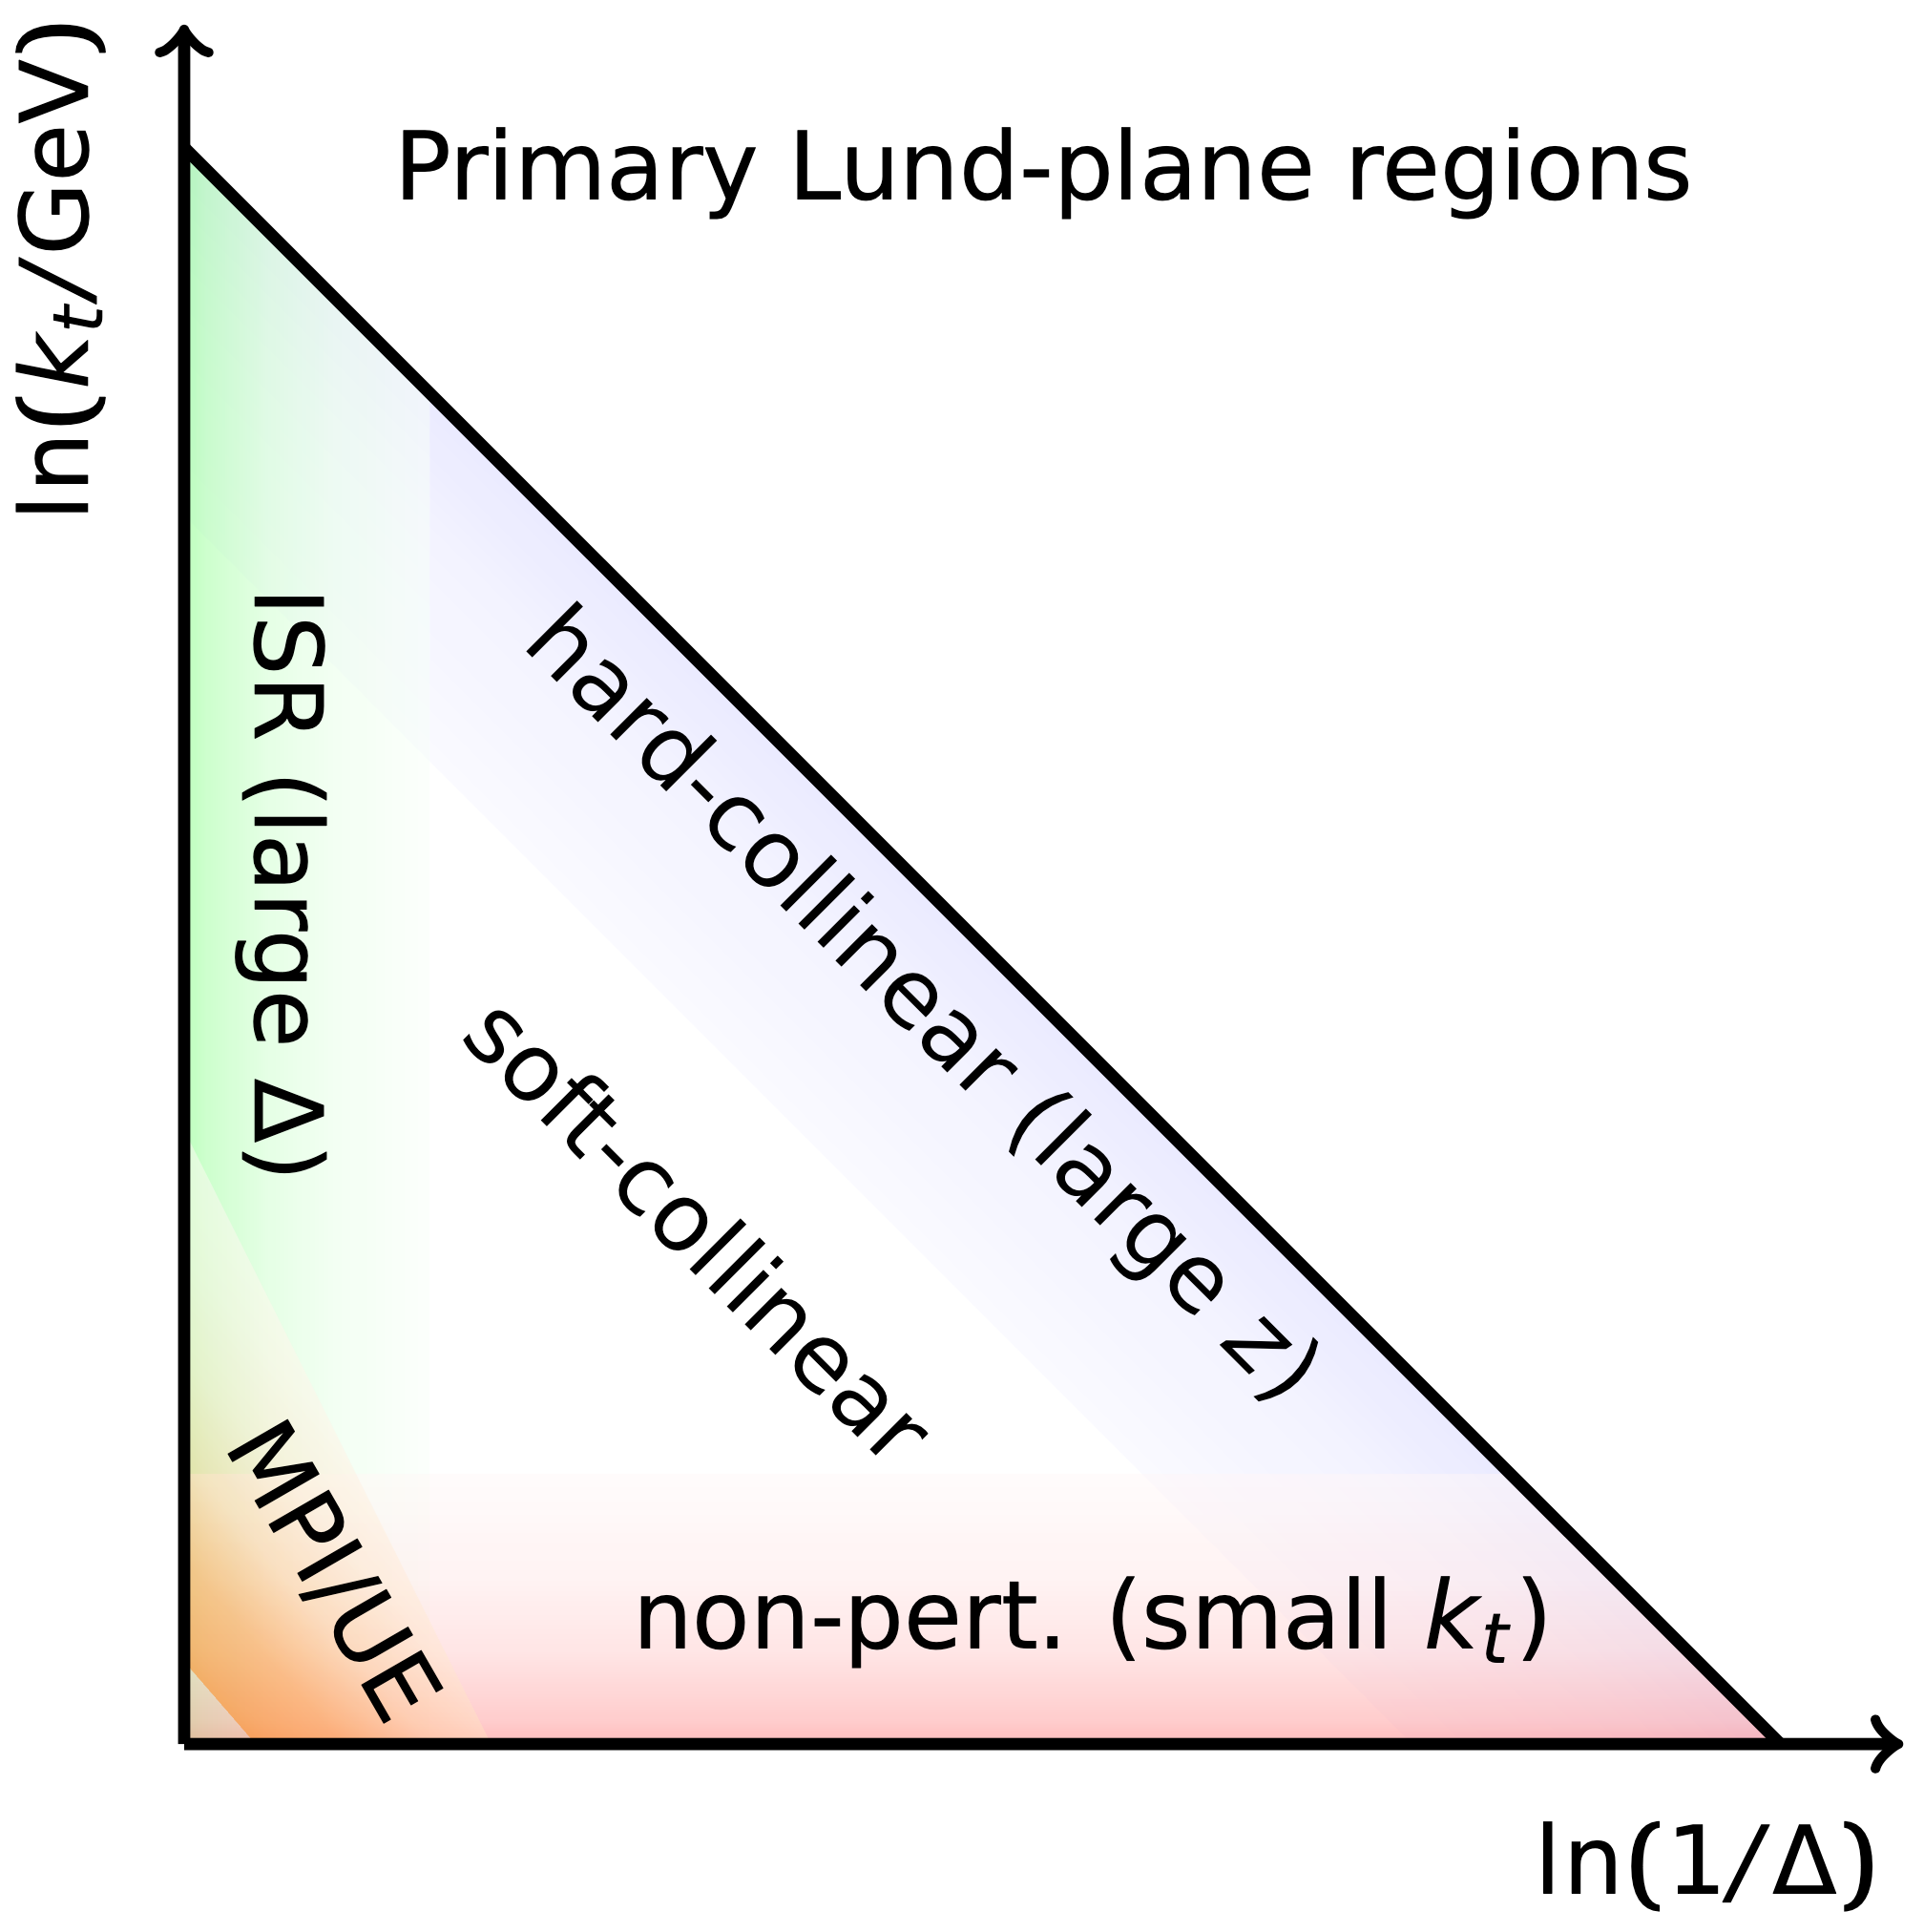
\includegraphics[width=0.25\textwidth]{figures/05-HH/part/lundplane.png}}
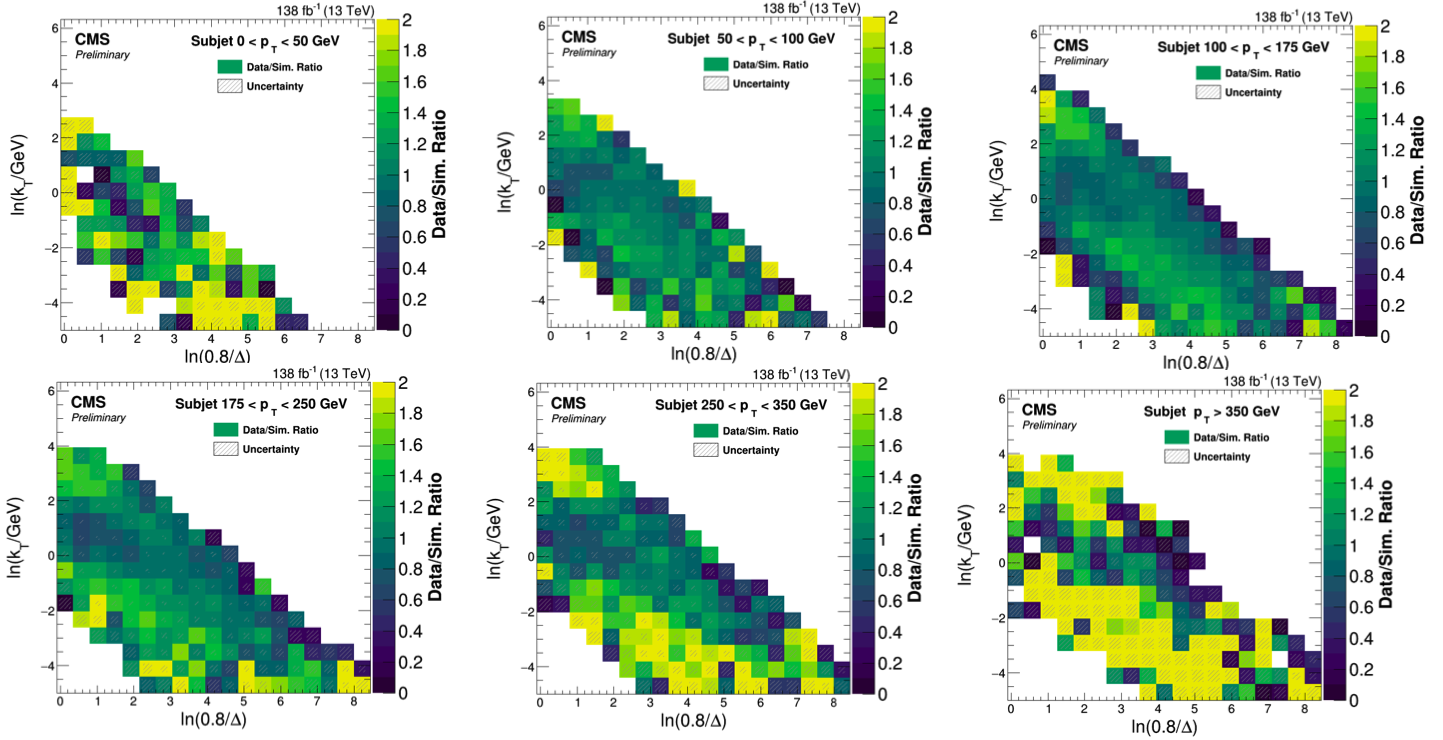
\includegraphics[width=0.74\textwidth]{figures/05-HH/part/lundratios.png}
\caption{Regions of the primary Lund plane (left) and data versus MC Lund plane ratios in $\PW\to\qqbar$ jets, binned in subjet \pt (right), reproduced from Refs.~\cite{Dreyer:2018nbf} and~\cite{CMS-DP-2023-046}, respectively.}
\label{fig:05_part_lundplane}
\end{figure}

A data-to-MC per-event relative weight for the signal is derived by calculating the primary Lund planes for each subjet in the \hvv jet, then taking the product across the subjets of each splitting's data-to-MC correction factor (from Figure~\ref{fig:05_part_lundplane}) as a function of its \kt, $\Delta$, and subjet \pt.
% These weights thus capture overall data/MC mismodeling based on the differences in each subjet's radiation pattern.
The signal efficiency scale factor for a BDT selection in the nonresonant analysis, and the \THWW selection in the resonant analysis, is thus defined as the ratio of the efficiencies before and after applying the Lund plane weights.
Statistical uncertainties and systematic uncertainties related to the MC modeling and extrapolation up to high \pt subjets on the data-to-MC Lund plane ratios are each propagated as sources of systematic uncertainties on the scale factor, as well as an additional factor representing the uncertainty on the quark-subjet matching, as described in detail in Ref.~\cite{CMS-DP-2023-046}.
The measured SFs and uncertainties for different signals and analysis regions are shown in Chapter~\ref{sec:05_hh_systematics}.

The scale factor measurement is validated for the GloParT on boosted top quark jets.
We define a semi-leptonic boosted \ttbar control region, tagging a leptonically-decaying top quark ($\PQt\to\PQb\PW\to\PQb\PGm\PGn$), and then probing an opposite-side high \pt AK8 jet representing the hadronically-decaying quark.
The event selection follows that of the control region in Ref.~\cite{CMS-DP-2023-046}, comprising online muon triggers, and offline selections for a \PQb-tagged AK4 jet, a leptonically-decaying \PW boson --- based on the presence of a muon and missing transverse energy --- and a high \pt AK8 jet with mass close to that of the top quark.
Jets from the \ttbar MC samples are categorized using generator-level particles as either: ``top matched'' --- all three daughter quarks lying within the jet; ``W matched'' --- only the \PW daughter quarks inside the jet; or ``unmatched'' --- neither of these two cases.
Only the top-matched jets are reweighted with the Lund plane ratios.

We consider the \THWW discriminant from Eq.~\ref{eq:05_thww}, excluding \PTop in the denominator to ensure top quark events are retained in the high tagger score bins.
Plots of the \THWW distribution from the 2018 datasets before and after Lund plane reweighting of the top-matched jets are shown in Figure~\ref{fig:05_part_ttbar}.
The combined uncertainties per bin are also shown in the distributions and data/MC ratios.
We observe an overall improvement in data/MC agreement in the highest \THWW bins ($\THWW > 0.6$), with the $\chi^2$-test value between MC and data yields improving from 16.6 to 10.9.
The data and MC yields are all consistent within $1\sigma$ in these bins.

\begin{figure}[hbt]
\centering
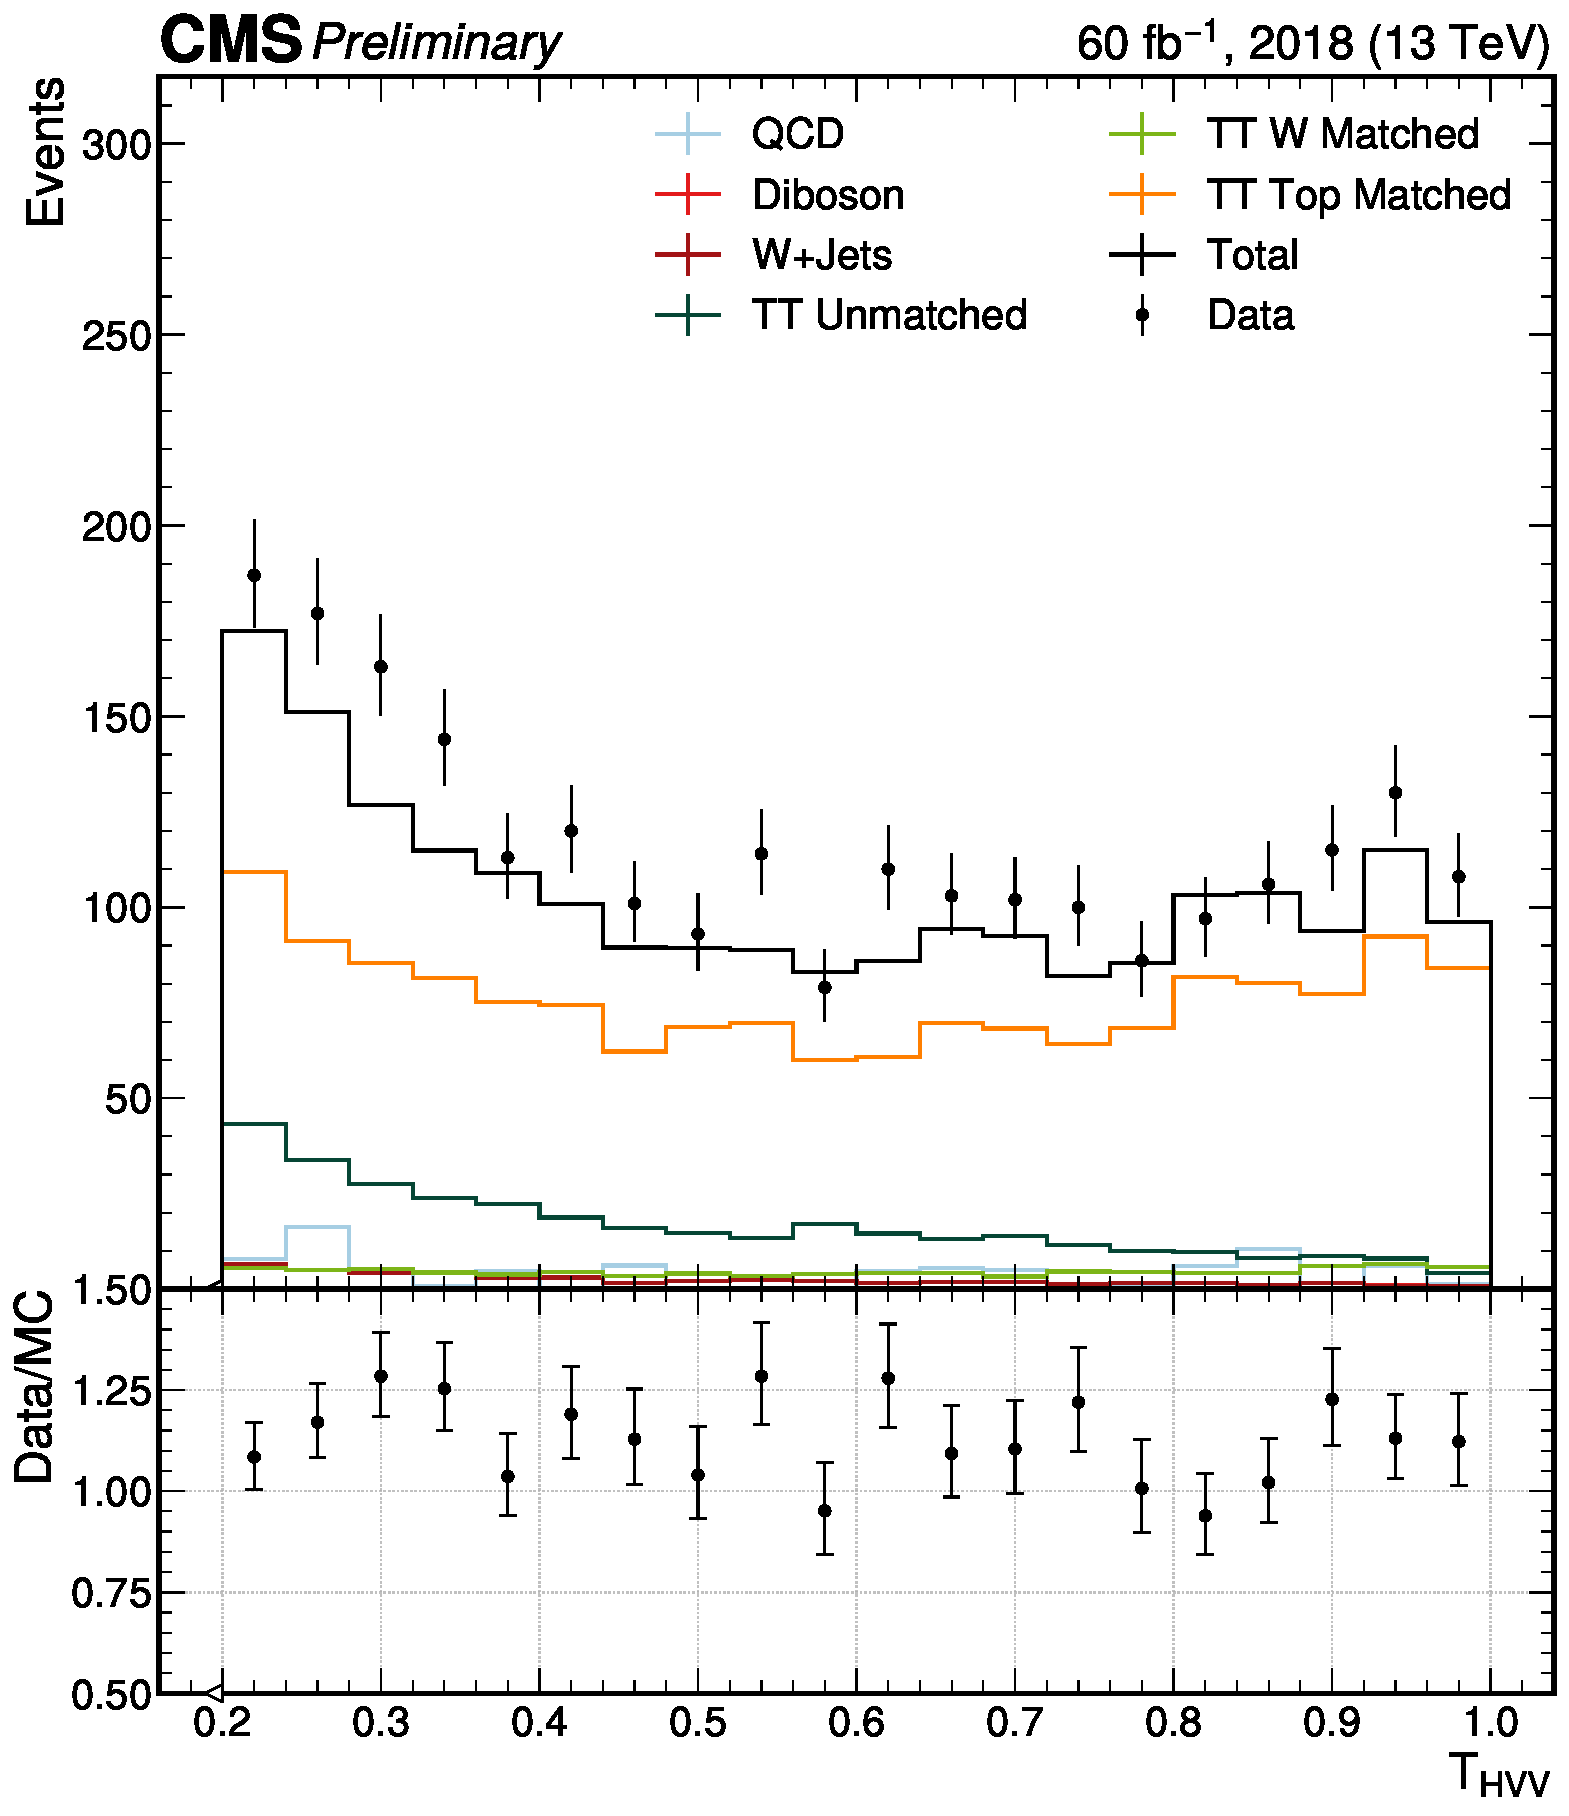
\includegraphics[width=0.49\textwidth]{figures/05-HH/part/pre_ak8FatJetParTMD_THWW4q-prelim.pdf}
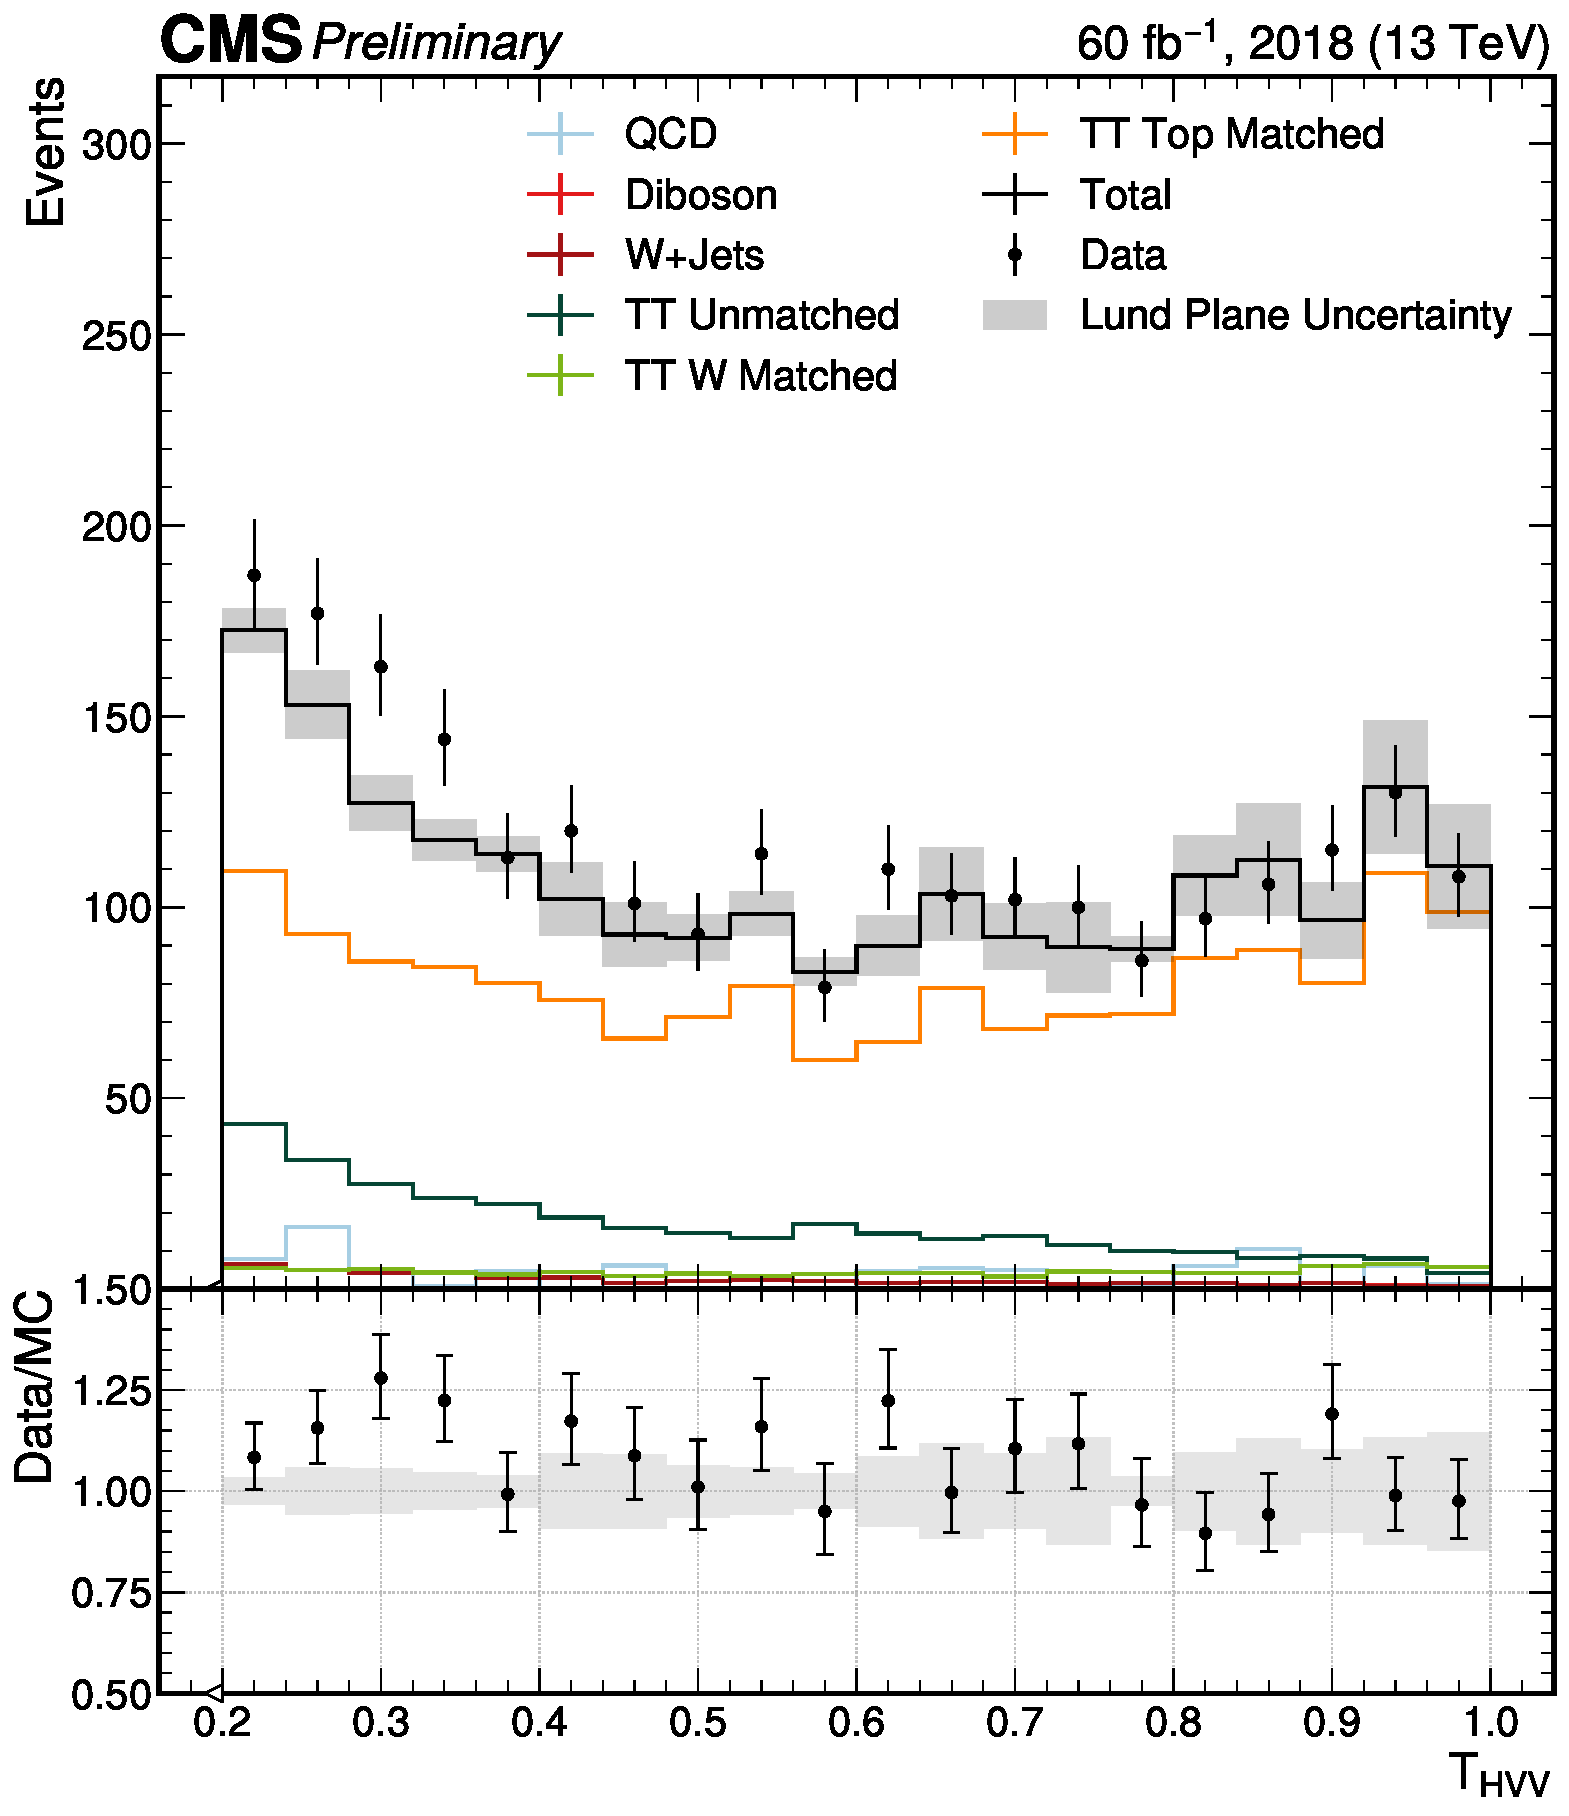
\includegraphics[width=0.49\textwidth]{figures/05-HH/part/postlnN_ak8FatJetParTMD_THWW4q-prelim.pdf}
\caption[Distributions of the GloParT \THWW discriminant before and after the Lund plane reweighting of top matched jets.]{Distributions of the GloParT \THWW discriminant before (left) and after (right) the Lund plane reweighting of top matched jets.
The combined uncertainties from Lund-plane-based scale factors on the MC yield per bin are shown in gray on the right.
\label{fig:05_part_ttbar}
}
\end{figure}

\subsubsection{Acknowledgements}

This chapter, in part, is currently being prepared for the publication of the material by the CMS collaboration.
The dissertation author was the primary investigator and author of these papers.
